\documentclass{article}
\usepackage{hyperref}
\usepackage{listings}
\usepackage{graphicx}
\usepackage{fancyhdr}
\usepackage{color}

\pagestyle{fancy}



\begin{document}


\begin{titlepage}
	\begin{center}
	\line(1,0){300}\\
	[0.25in]
	\huge\bfseries\ Programming Project 2 \\Napster-style peer-to-peer (P2P) file sharing system \\
	
	
	\line(1,0){250}\\
	\bfseries {Geoffrey Rathinpandi}\\
	\end{center}
	
	

	\begin{flushright}
	\textsc{R11488765}\\
	
	
	\end{flushright}
	\tableofcontents
\end{titlepage}
\section{GithubLink}
The github link :  \url{https://github.com/Ge0f3/Peer2Peer } \\ \\

\section{Overview}

This project aims to provide a coordinator server that store and process file
indexes of peers, which are pre-registered by peers. Moreover, those stored indexes may be shared with peers ,with location information, based on a peer request. On the other hand, peers in this system have the ability to register and downloads files. The system accept N number of peers since the server is using a multi-threaded listeners.


\section{Work Flow}

The work flow of the project  \\

\begin{figure} [h]
\centering
        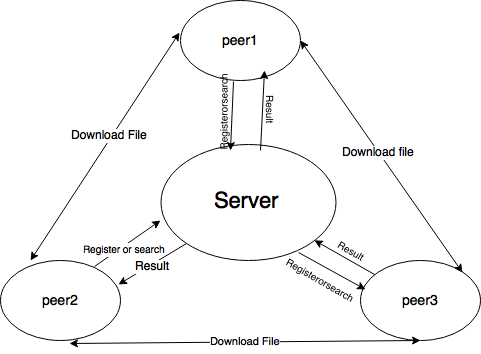
\includegraphics[totalheight=8cm]{workflow.png}
    \caption{Workflow}
    \label{fig:verticalcell}
\end{figure}
\section{Architecture}
\begin{itemize}
\item Indexing Server Architecture :
\begin{itemize}
\item Indexing server is the entity that stores the files indexes which are registered by
peers. It is the heart of the system that provides all the information from peers to
download files.
\item The server stores indexes in a concurrent hash table which uses the filename as an
ID and an array content.
\item The array holds the messages object.
\item Each message contains a peer information (IP, port, command..).
\item This hash map can be accessed by many threads in order to lookup. However, it
will be blocked if there a writing operation on it.
\item The server listens for peers all the time. The port ‘60000’ is reserved for registration requests while port ‘60001’ is reserved for lookup requests.
\item Once a request is received, the server will accept the connection immediately and create new thread to handle that request.
\end{itemize}
\item Peer Architecture :
\begin{itemize}
\item Each peer has three major functionality, listening to other peer, making request to
the server, and requesting from another peer.
\item In term to get a file from a peer, a peer should be listening to others requests, and
send the requested files to them.
\item Searching a file required user input to get the required file name, and returns list of (peer id and IP), which is the locations that a file existed
\item Register a file allow user to register a file index in the server. It is requires the file name, and this file should be existed on the current machine.
Register all files, allows the user to register all the files existed on the resources folder.
\item Download file from a peer, allows user to get a file from another peer. It requires the user to type the peer ID, IP, and the file name in this format (pppp-IP-filename.ext).
\item List my files, displays the files which are on the resources folder, to the user.
Calculate the performance, let the user measure the search request performance using N number of requests. It requires the file name and the number of needed
search request, and return time in milliseconds. \\ \\ \\
\end{itemize}
\end{itemize}

\section{Functionality of peers}
The functionality provided for the peers is mentioned below in the figure
\begin{figure} [h]

        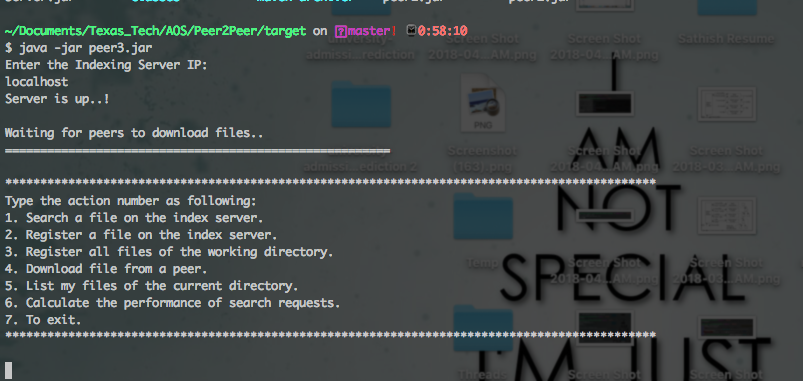
\includegraphics[totalheight=8cm]{Func.png}
    \caption{Functionality of peers}
    \label{fig:verticalcell}
\end{figure}

\section{Future Enhancement}
\begin{itemize}
\item Enhancing the performance by apply load balancing approach on the server side.
\item Dynamic ports allocation needed in the system to avoid overlapping reserved
ports.
\item A simple GUI will make it user friendly.

\end{itemize}





\end{document}